\documentclass[final,twoside]{rapport}  % options [chapter,final]
\usepackage{schoolbook,graphicx,paperhead,tabularx,manual,psfrag,verbatim}

\DeclareMathOperator{\E}{E\,}
\DeclareMathOperator{\Prob}{Prob\,}
\DeclareMathOperator{\U}{U}

\bibliographystyle{LongLabels}

\begin{document}

\thispagestyle{empty}
\setlength{\parindent}{0pt}
\setlength{\parskip}{1em plus 0.1em minus 0.1em}
%\addtolength{\oddsidemargin}{-1em}

\begin{paperhead}
\vspace{-1cm}
\title{Course on Embedded Real-Time
  Computing and Control\\[1em]Computer Exercise on Jitterbug}
\author{}
\end{paperhead}

\vspace*{-2.5cm}

\subsection*{Introduction}

Jitterbug is a Matlab toolbox for stochastic performance analysis of
control systems with random delays. A control system is described by
two parallel models: a signal model and a timing model. The signal
model is given by a number of connected, linear, continuous- and
discrete-time systems disturbed by white noise. The timing model
consists of a number of timing nodes and describes when the different
discrete-time systems should be updated during the control period.
The toolbox analytically evaluates an analytical performance index in
the form
\[
J = \E x^T Q x
\]
where the vector $x$ collects all states in the model and $Q$ is a
weighting matrix.

\subsection*{First example -- \texttt{kushner.m}}

We start by studying a classical example from  Kushner \& Kushner
(1969)\footnote{H.J. Kushner, L. Tobias: ``On the stability of
  randomly sampled systems''. {\em IEEE Transactions on Automatic
    Control}, Vol AC-14, No. 4, August 1969}, where it is shown that
{\em sampling jitter can actually
increase 
the control performance in some cases}. The signal and timing models
are shown below:
\bigskip

  \centerline{
    \small
  \psfrag{G(s)}[c][c]{$P(s)$}
  \psfrag{H2}[c][c]{$C(z)$}
  \psfrag{S}[c][c]{$\Sigma$}
  \psfrag{y}[c][c]{$y$}
  \psfrag{u}[c][c]{$u$}
  \psfrag{v}[c][c]{$v_c$}
  \psfrag{n1}[c][c]{$1$}
  \psfrag{n2}[c][c]{$2$}
  \psfrag{t1}[c][c]{$\tau$}
  \psfrag{(a)}[c][c]{\small (a)}
  \psfrag{(b)}[c][c]{\small (b)}
  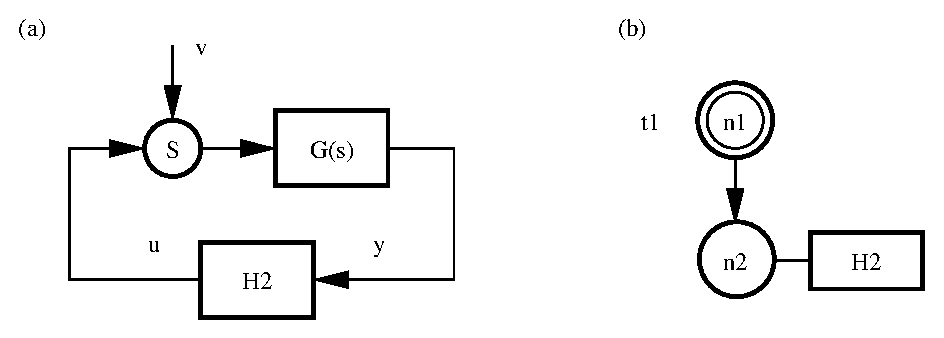
\includegraphics[scale=0.63]{kushner.eps}
  }

The system to be controlled is a stable second-order system, $P(s) =
\frac{6}{(s+1)(s+2)}$, that is disturbed by white noise $v_c$ with
unit intensity. The system is controlled by a simple P-controller,
$C(z) = -1$, with the nominal sampling interval $h=1.42$. The
performance is measured by the process output variance, $J= \E y^2$.
Sampling jitter is modelled by a periodic timing model with two
nodes. The first node represents the start of the period (indicated by
the extra ring). After a random delay $\tau$, the second node is
activated, triggering the controller system $C(z)$. When $C(z)$ is
triggered, the measurement signal $y$ is sampled and the control
signal $u\, (=-y)$ is updated.

Below, we walk through the details of the script. We start by defining the systems and the noise and cost matrices in
Matlab:
\begin{small}
\begin{verbatim}
s = tf('s');          % Define the Laplace transform variable s
P = 6/((s+1)*(s+2));  % Define the plant
C = -1;               % Define the controller (unit negative feedback)
R1 = 1;               % Input noise intensity
R2 = 0;               % Measurement noise variance
Q = diag([1 0]);      % Cost function: J = E (y^2 + 0 u^2)
\end{verbatim}
\end{small}

Next, we initialize the Jitterbug computation, specifying the period $h$
of the timing model and the time grain $\delta$ of the delay distributions. All
model data is stored in the local variable $N$:

\begin{small}
\begin{verbatim}
h = 1.42;                    % Period of timing model
delta = h/50;                % Time-grain
N = initjitterbug(delta,h);  % Initialize Jitterbug
\end{verbatim}
\end{small}


The random sampling delay $\tau$ is described by a
discrete-time probability density function
\begin{equation*}
P_\tau = \begin{bmatrix} P_\tau(0) & P_\tau(1) & P_\tau(2) & \ldots
\end{bmatrix},
\end{equation*}
where $P_\tau(k)$ represents the probability of a delay of
$k\delta$ seconds. A uniform delay between 0 and $L$ is hence
represented by a vector
\[
P_\tau = \begin{bmatrix}\smash{\underbrace{\tfrac{1}{d} \   \tfrac{1}{d} \
    \ldots \ 
  \tfrac{1}{d}}_{d \text{ elements}}} & 0 & \ldots \end{bmatrix}
\bigskip
\] 
where $d = 1+ L/\delta$. In Matlab, this can be entered as
\begin{small}
\begin{verbatim}
Ptau = ones(1,1+round(L/dt));  % Uniform delay between 0 and L
Ptau = Ptau/sum(Ptau);
\end{verbatim}
\end{small}
We are now ready to add the two timing nodes to the model:
\begin{small}
\begin{verbatim}
N = addtimingnode(N,1,Ptau,2);   % Add node 1 (the periodic node)
N = addtimingnode(N,2);          % Add node 2
\end{verbatim}
\end{small}
The timing nodes are numbered from 1 and upwards. The fourth argument
to {\tt addtimingnode} specifies which node to activate next.

Next, we build the signal model. The systems are also numbered
from 1 and up. For each system, it must be specified from which system
the input should be taken. Cost and noise matrices are optional
arguments. For the discrete system we specify that it should be executed in timing node 2:
\begin{small}
\begin{verbatim}
N = addcontsys(N,1,P,2,Q,R1,R2); % Add sys 1 (P), input from sys 2
N = adddiscsys(N,2,C,1,2);       % Add sys 2 (C), input from sys 1, exec in 2 
\end{verbatim}
\end{small}
Finally, the cost $J$ is computed using the commands
\begin{small}
\begin{verbatim}
N = calcdynamics(N);             % Calculate the internal dynamics
J = calccost(N)                  % Calculate the cost
\end{verbatim}
\end{small}

\subsubsection{Assignment 1.}

Run the script \texttt{kushner.m }and study the resulting plot. What
is the best value of the sampling jitter? For what jitter does the
system go unstable?

\subsubsection{Assignment 2.}

Modify the script in order to investigate if {\em input-output jitter}
can also have a stabilizing effect. You will need to insert an additional
discrete-time system $S(z)=1$ that represents the sampler. You also have
to change the timing model to reflect that the sampler should execute
at the start of the period, and the controller after the delay $\tau$,
see below.

\bigskip

  \centerline{
    \small
  \psfrag{G(s)}[c][c]{$P(s)$}
  \psfrag{H1}[c][c]{$S(z)$}
  \psfrag{H2}[c][c]{$C(z)$}
  \psfrag{S}[c][c]{$\Sigma$}
  \psfrag{y}[c][c]{$y$}
  \psfrag{u}[c][c]{$u$}
  \psfrag{v}[c][c]{$v_c$}
  \psfrag{n1}[c][c]{$1$}
  \psfrag{n2}[c][c]{$2$}
  \psfrag{t1}[c][c]{$\tau$}
  \psfrag{(a)}[c][c]{\small (a)}
  \psfrag{(b)}[c][c]{\small (b)}
  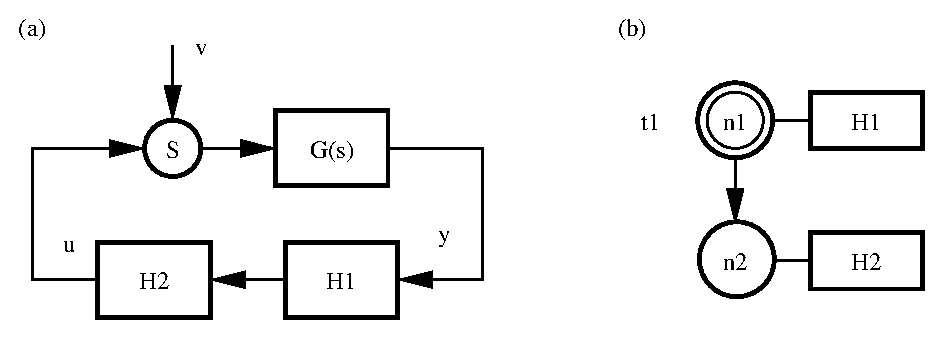
\includegraphics[scale=0.63]{kushner2.eps}
  }

Run your modified script and study the resulting plot. For what value
of input-output jitter is the minimum cost achieved?

\medskip
\subsection*{Second example -- \texttt{simple.m}}

Jitter in the control output can be removed by introducing a buffer
and a dedicated output task. This however increases the input-output
delay. The question is, which is worse, jitter or delay?

Based on the script \texttt{simple.m}, perform an investigation with
the following input data:

\begin{itemize}
\item Plant: $P(s) = \frac{1}{s(s+1)}$ (DC servo)
\item Input noise: $R_{1c} = 1$, measurement noise $R_2 = 0.001$
\item Cost function: $J = \E \Bigl( y^2 + 0.001 u^2 \Bigr)$
\item Sampling interval and time grain: $h = 0.1$, $\delta = 0.01$
\end{itemize}

By changing the LQG design and the input-output delay distribution,
compare the resulting cost in the following four cases:
\begin{enumerate}
\item Zero delay; LQG controller designed for zero delay
\item Uniform delay between 0 and $h$; LQG controller designed for zero delay
\item Uniform delay between 0 and $h$; LQG controller designed for
  average delay 
\item Constant delay $h$; LQG controller designed for delay $h$
\end{enumerate}
Case 1 is only used as a reference. Which of the implementation
alternatives  2--4 gives the best performance in this case?

\end{document}